% IMPORTANT NOTES TO FOLLOW OVERALL:
%A) the lab description of the respective topic (to make the report selfcontained)
%B) 1-2 pages pointing out how much they solved and which issues they encountered
%C) A “print” of an example run
%D) 1-2 pages where they relate what they did to the relevant theory in the curriculum
%E) max 1 page conclusion, concluding what was solved well (perhaps even makes you proud :-)- and what could be done differently/better and why

\section*{Secure Task Manager}

\subsection*{Description}

The objective of this chapter is to implement a simple security protocol for our task manager. We have been developing a simple role based access control mechanism for tasks based on an authentication using ITU credentials. Moreover, we have been using one of the crypto algorithms to ensure security among all/some parts of communication.

Furthermore, in order to support role based access controls for tasks,  the task-manager-revised.xml has been updated with a role on the task element.

\begin{figure}[ht!]
	\centering
		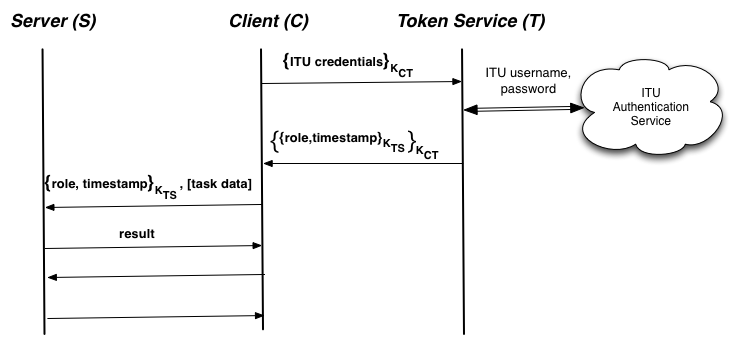
\includegraphics[width=90mm]{graphics/task-manager-security-protocol.png}
		\caption{Task Manager Security Protocol}
		\label{overflow}
\end{figure}
%figure: improved security model from lab description

There are 3 interacting principals offering  the same functionality. But the communication between different principals is encrypted with keys shared in between them. The three principals are:

\subsubsection*{Token Service:} It authenticates clients’s credentials (ITU username and password). Furthermore, the token service also maintains authorization of tasks by having role mappings for a given ITU user account that matches to the roles assigned to the tasks in the task-manager-revised.xml. On successful validation  of client’s credentials, the token service will generate an encrypted server token containing client’s role, timestamp, client’s name and a encryption key for sharing between client and server (K_SC). In addition to the server token, the token service will also send the encryption key (K_SC).

\subsubsection*{Server:} The server offers two functions: authenticate and execute. The client will first authenticate itself by sending the server token. On successful authentication, the server will generate a nonce (N) and send it to the client. On the other hand, in case of authentication failure, the server provides error message only.
 
Client: The client first contacts the token service by proving ITU username and password, to receive the double encrypted server token. First, it decrypts the server token with its key shared with token service (K_CT), to extract the encrypted server token. Then it will send the encrypted server token along with task data to server for executing  the tasks of the task manager.



\subsection*{Implementation}

implementation will go here:



\subsection*{Related Theory}

Unlike SOAP with ws-secure, REST does not come with a security protocol. But as any web application the 
Rest services also nee to be secure. The question is which threats are we concerned about, and how can we beat these. 

We will have to assume that there is a mischievous person, who will attempt to read, remember, intercept, interrupt, modify and fabricate messages. 

Design security protocols using:
\begin{itemize}
	\item Cryptography
	\item Authentication
	\item Secure channels
\end{itemize}
 
When building web applications and services it is wise to predict worst case assumptions:
\begin{itemize}
	\item Exposed interfaces
	\item Insecure networks
	\item Secrets between many participants hard to be kept for a long period
	\item Algorithms and code known to enemy
	\item Enemy has access to large resources
\end{itemize}

Security mechanisms:
\begin{itemize}
	\item Cryptography
	\item Certificates
	\item Access control
	\item Credentials
	\item Firewalls
\end{itemize}


Even though REST doesn't come with a dedicated security protocol, there are external protocols that are recommended to use together with REST instead if implementing your own. OAuth is one popular choice. OAuth is an open protocol to allow secure authorization in a simple and standard method from web, mobile and desktop applications. The OAuth 2.0 authorization framework enables a third-party application to obtain limited access to an HTTP service.

\subsection*{Conclusion}

